\documentclass{article}
\usepackage{122}

\usepackage{array}
\usepackage{graphicx}
\usepackage[hidelinks,bookmarks=false]{hyperref}
\usepackage{attachfile2}

\title{Биоинформатика \\ Домашнее задание №2}

\graphicspath{ {../bio/RNA polymerase RPB3/screenshots/} }
\newcolumntype{C}{ >{\centering\arraybackslash} m{.3\textwidth} }

\begin{document}
  \maketitle

  \section{Выбранный ген}
  \texttt{RNA polymerase RPB3} более извесный как \\
  \texttt{DNA-directed RNA polymerase II subunit RPB3} или \\
  \texttt{DNA-directed RNA polymerase II subunit С}

  \section{Скачанные последовательности}
  Я скачивал все гены с uniprot-а и всего их получилось 23.
  Растений, бактерий и архей мне не удалось найти, так как этот ген есть только у эукариот
  <<This gene encodes the third largest subunit of RNA polymerase II, the polymerase responsible for synthesizing messenger RNA in eukaryotes.>>
  [\href{https://en.wikipedia.org/wiki/POLR2C}{Wikipedia}].
  В этой таблице также есть вложенные файлы, которые теоретически можно скачать double click-ом в некоторых pdf reader-ах.

  \begin{center}
    \begin{tabular}{|c|l|l|l|l|}
      \hline
      № & Латинское таксономическое название & Английское название & ссылка на uniprot & файл
      \\\hline
      1 &Lygus hesperus & lygus bug & \href{https://www.uniprot.org/uniprot/A0A0A9ZDH0}{\texttt{A0A0A9ZDH0}} & \attachfile{../bio/RNA polymerase RPB3/fasta/A0A0A9ZDH0.fasta} \\
      2 &Trichinella murrelli & nematodes & \href{https://www.uniprot.org/uniprot/A0A0V0TF24}{\texttt{A0A0V0TF24}} & \attachfile{../bio/RNA polymerase RPB3/fasta/A0A0V0TF24.fasta} \\
      3 &Trichinella sp. T8 & nematodes & \href{https://www.uniprot.org/uniprot/A0A0V1PGK5}{\texttt{A0A0V1PGK5}} & \attachfile{../bio/RNA polymerase RPB3/fasta/A0A0V1PGK5.fasta} \\
      4 &Hanseniaspora opuntiae & budding yeasts & \href{https://www.uniprot.org/uniprot/A0A1E5RMS7}{\texttt{A0A1E5RMS7}} & \attachfile{../bio/RNA polymerase RPB3/fasta/A0A1E5RMS7.fasta} \\
      5 &Lonchura striata domestica & Bengalese finch & \href{https://www.uniprot.org/uniprot/A0A218V770}{\texttt{A0A218V770}} & \attachfile{../bio/RNA polymerase RPB3/fasta/A0A218V770.fasta} \\
      6 &Macaca fascicularis & crab-eating macaque & \href{https://www.uniprot.org/uniprot/A0A2K5UGS4}{\texttt{A0A2K5UGS4}} & \attachfile{../bio/RNA polymerase RPB3/fasta/A0A2K5UGS4.fasta} \\
      7 &Neophocaena asiaeorientalis asiaeorientalis & Yangtze finless porpoise & \href{https://www.uniprot.org/uniprot/A0A341BKL9}{\texttt{A0A341BKL9}} & \attachfile{../bio/RNA polymerase RPB3/fasta/A0A341BKL9.fasta} \\
      8 &Callorhinus ursinus & northern fur seal & \href{https://www.uniprot.org/uniprot/A0A3Q7QGL8}{\texttt{A0A3Q7QGL8}} & \attachfile{../bio/RNA polymerase RPB3/fasta/A0A3Q7QGL8.fasta} \\
      9 &Vombatus ursinus & common wombat & \href{https://www.uniprot.org/uniprot/A0A4X2LNH6}{\texttt{A0A4X2LNH6}} & \attachfile{../bio/RNA polymerase RPB3/fasta/A0A4X2LNH6.fasta} \\
      10 &Camelus dromedarius & Arabian camel & \href{https://www.uniprot.org/uniprot/A0A5N4DQV9}{\texttt{A0A5N4DQV9}} & \attachfile{../bio/RNA polymerase RPB3/fasta/A0A5N4DQV9.fasta} \\
      11 &Acinonyx jubatus & cheetah & \href{https://www.uniprot.org/uniprot/A0A6J2ASW7}{\texttt{A0A6J2ASW7}} & \attachfile{../bio/RNA polymerase RPB3/fasta/A0A6J2ASW7.fasta} \\
      12 &Harpegnathos saltator & Jerdon's jumping ant & \href{https://www.uniprot.org/uniprot/E2BRN1}{\texttt{E2BRN1}} & \attachfile{../bio/RNA polymerase RPB3/fasta/E2BRN1.fasta} \\
      13 &Sus scrofa & pig & \href{https://www.uniprot.org/uniprot/I3LCH3}{\texttt{I3LCH3}} & \attachfile{../bio/RNA polymerase RPB3/fasta/I3LCH3.fasta} \\
      14 &Bos mutus & wild yak & \href{https://www.uniprot.org/uniprot/L8IE22}{\texttt{L8IE22}} & \attachfile{../bio/RNA polymerase RPB3/fasta/L8IE22.fasta} \\
      15 &Tupaia chinensis & Chinese tree shrew & \href{https://www.uniprot.org/uniprot/L9KTQ2}{\texttt{L9KTQ2}} & \attachfile{../bio/RNA polymerase RPB3/fasta/L9KTQ2.fasta} \\
      16 &Chelonia mydas & Green sea turtle & \href{https://www.uniprot.org/uniprot/M7B5V7}{\texttt{M7B5V7}} & \attachfile{../bio/RNA polymerase RPB3/fasta/M7B5V7.fasta} \\
      17 &Saccharomyces cerevisiae & baker's yeast & \href{https://www.uniprot.org/uniprot/P16370}{\texttt{P16370}} & \attachfile{../bio/RNA polymerase RPB3/fasta/P16370.fasta} \\
      18 &Homo sapiens & human & \href{https://www.uniprot.org/uniprot/P19387}{\texttt{P19387}} & \attachfile{../bio/RNA polymerase RPB3/fasta/P19387.fasta} \\
      19 &Schizosaccharomyces pombe & fission yeast & \href{https://www.uniprot.org/uniprot/P37382}{\texttt{P37382}} & \attachfile{../bio/RNA polymerase RPB3/fasta/P37382.fasta} \\
      20 &Mus musculus & house mouse & \href{https://www.uniprot.org/uniprot/P97760}{\texttt{P97760}} & \attachfile{../bio/RNA polymerase RPB3/fasta/P97760.fasta} \\
      21 &Drosophila pseudoobscura pseudoobscura & flies & \href{https://www.uniprot.org/uniprot/Q29K78}{\texttt{Q29K78}} & \attachfile{../bio/RNA polymerase RPB3/fasta/Q29K78.fasta} \\
      22 &Bos taurus & cattle & \href{https://www.uniprot.org/uniprot/Q3T0Q3}{\texttt{Q3T0Q3}} & \attachfile{../bio/RNA polymerase RPB3/fasta/Q3T0Q3.fasta} \\
      23 &Dictyostelium discoideum & cellular slime molds & \href{https://www.uniprot.org/uniprot/Q54DH7}{\texttt{Q54DH7}} & \attachfile{../bio/RNA polymerase RPB3/fasta/Q54DH7.fasta} \\
      \hline
    \end{tabular}
  \end{center}

  \section{Скриншоты выравнивания}
  \subsection{Метод ClustalW}
  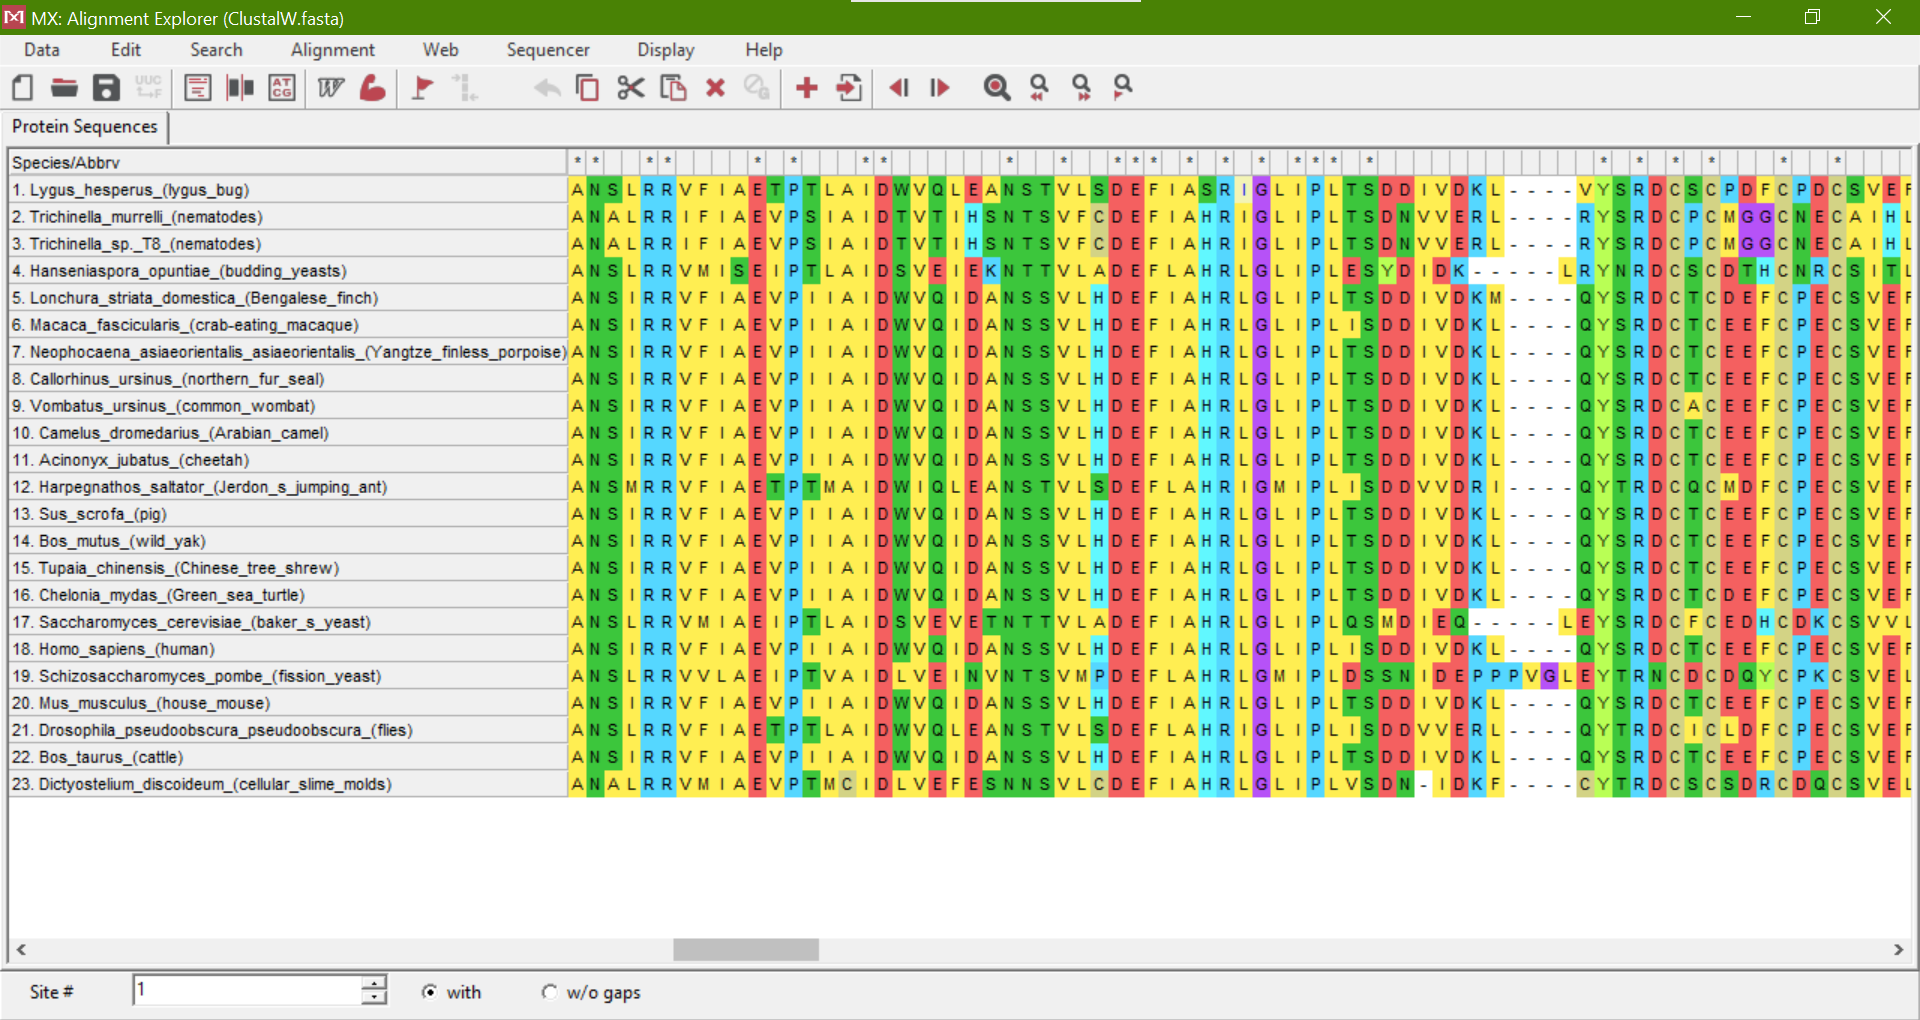
\includegraphics[width=\textwidth]{ClustalW.png}
  \subsection{Метод Muscle}
  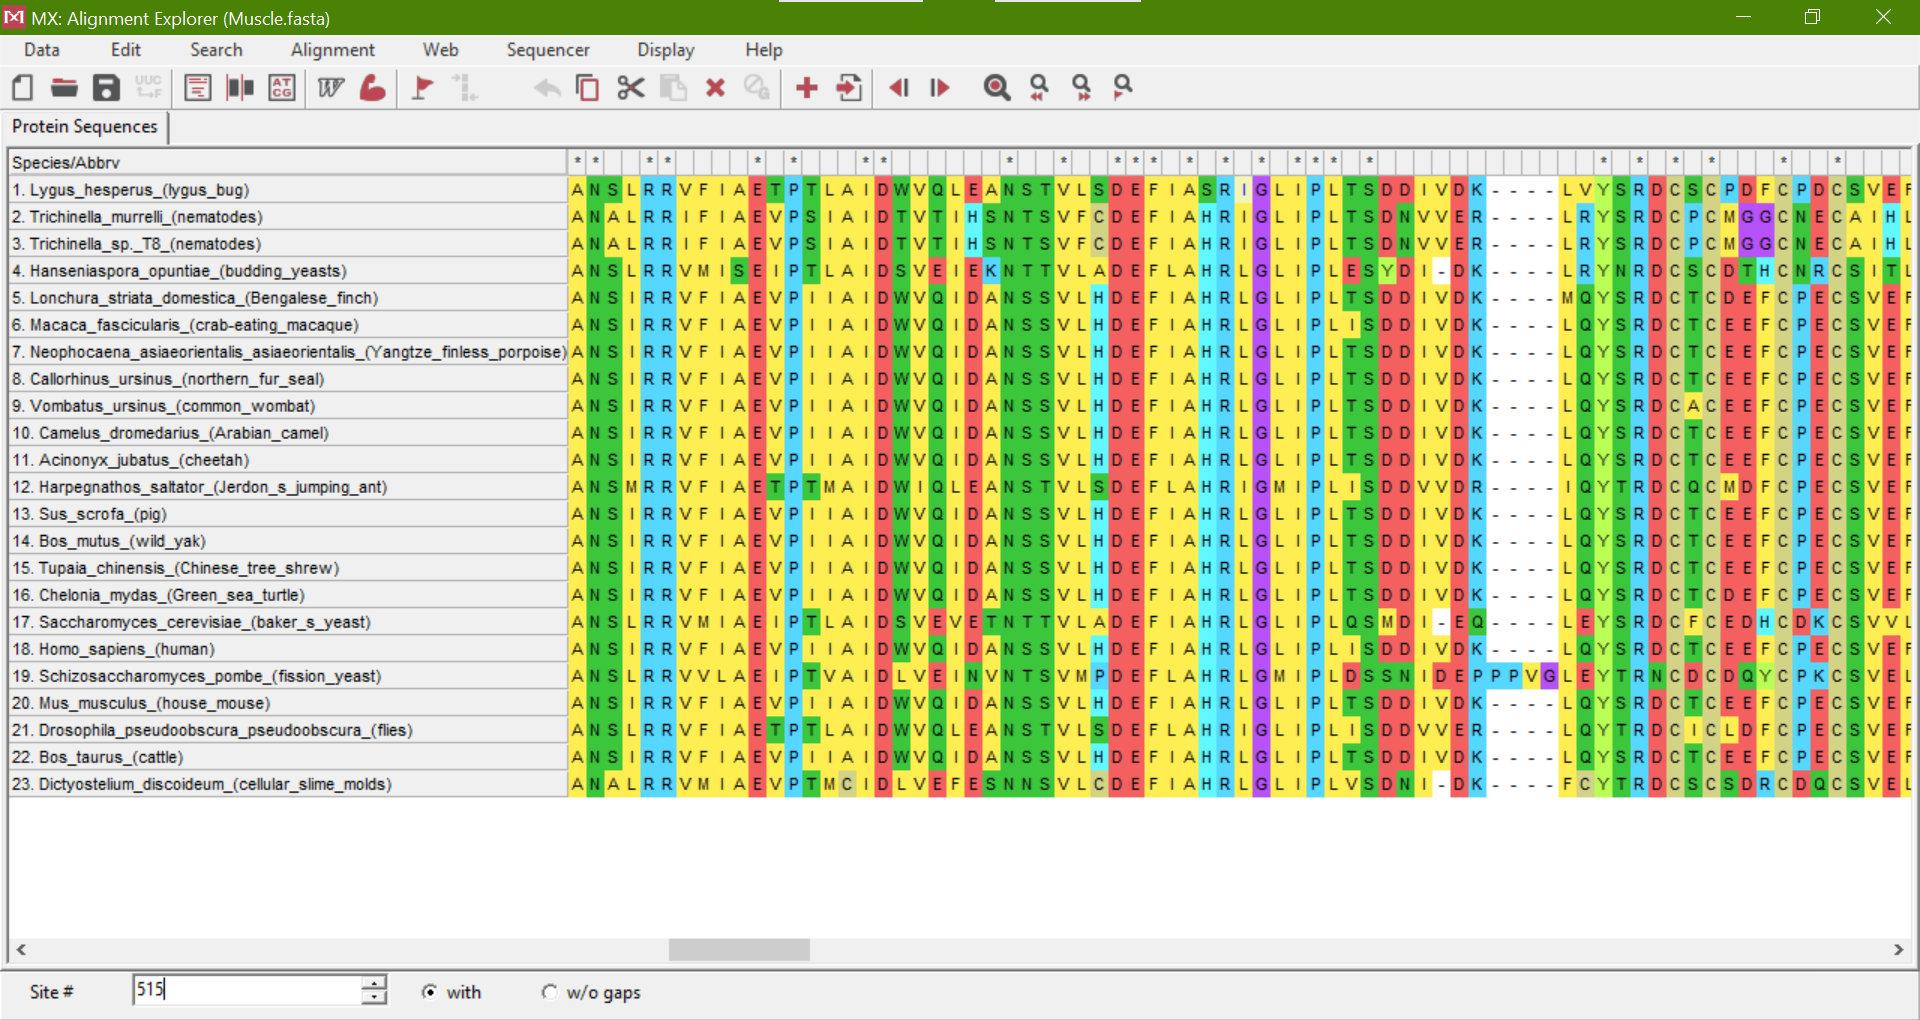
\includegraphics[width=\textwidth]{Muscle.png}

  \section{Скриншоты деревьев}
  \subsection{Метод выравнивания ClustalW}
  \begin{center}
    \begin{tabular}{|C|C|C|}
      \hline
      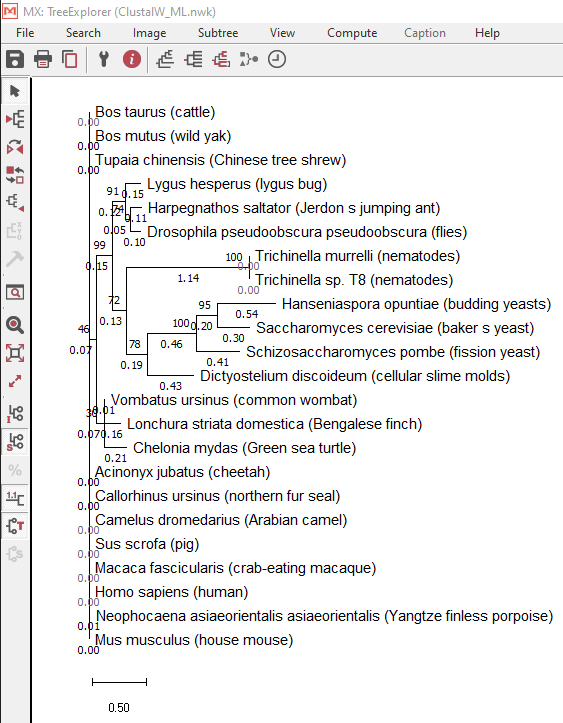
\includegraphics[width=.3\textwidth]{ClustalW_ML.png} &
      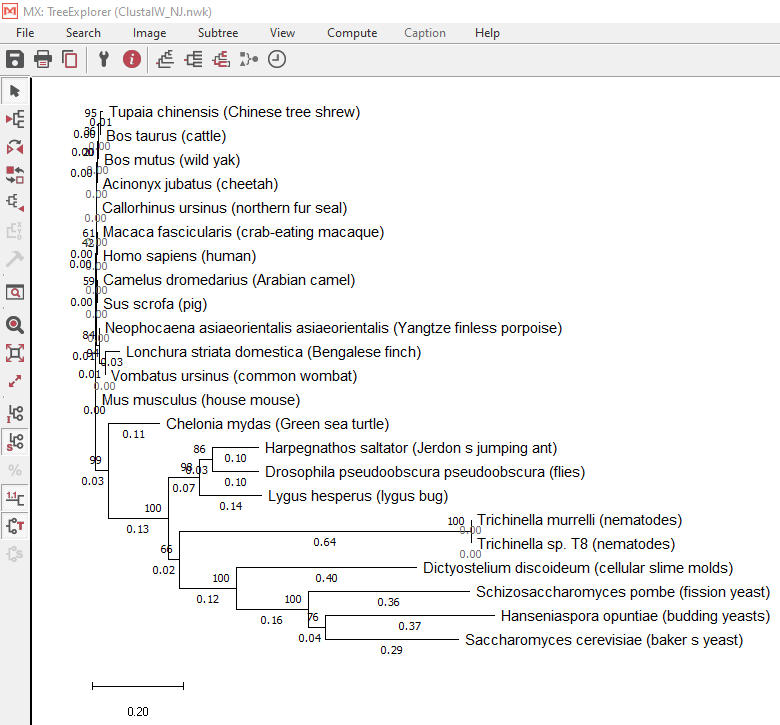
\includegraphics[width=.3\textwidth]{ClustalW_NJ.png} &
      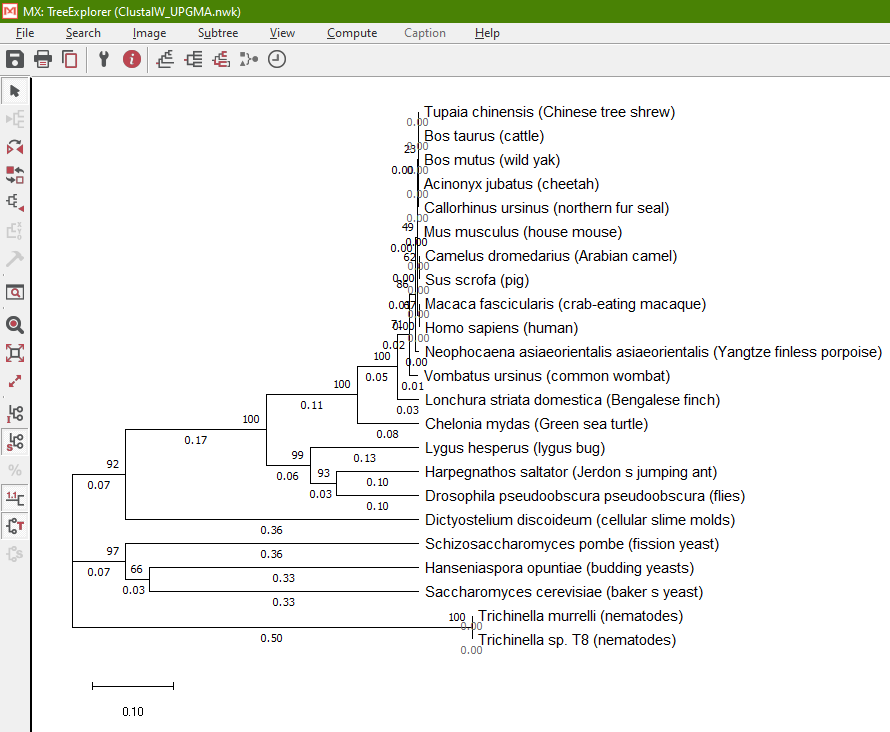
\includegraphics[width=.3\textwidth]{ClustalW_UPGMA.png} \\\hline
      Метод ClustalW и ML &
      Метод ClustalW и NJ &
      Метод ClustalW и UPGMA \\\hline
    \end{tabular}
  \end{center}

  \subsection{Метод выравнивания Muscle}
  \begin{center}
    \begin{tabular}{|C|C|C|}
      \hline
      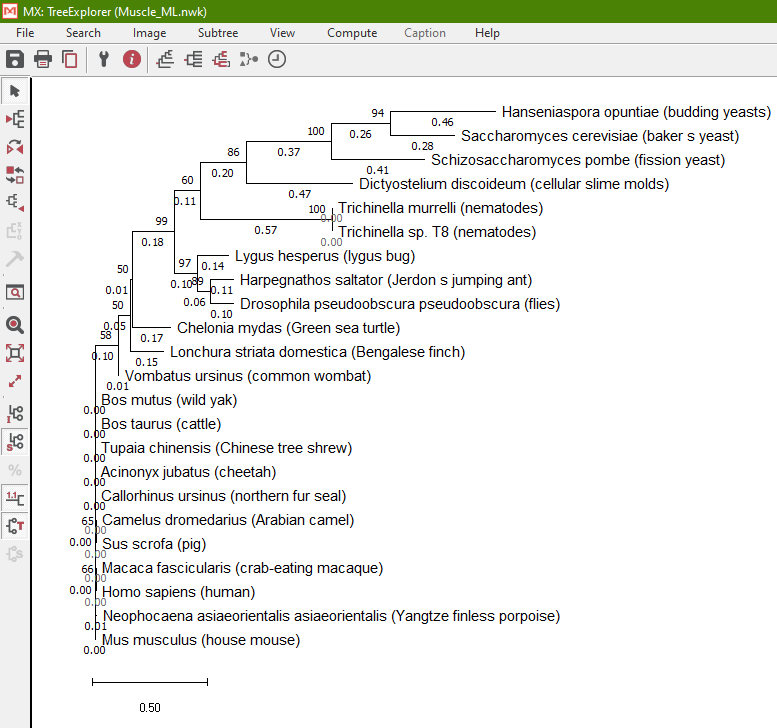
\includegraphics[width=.3\textwidth]{Muscle_ML.png} &
      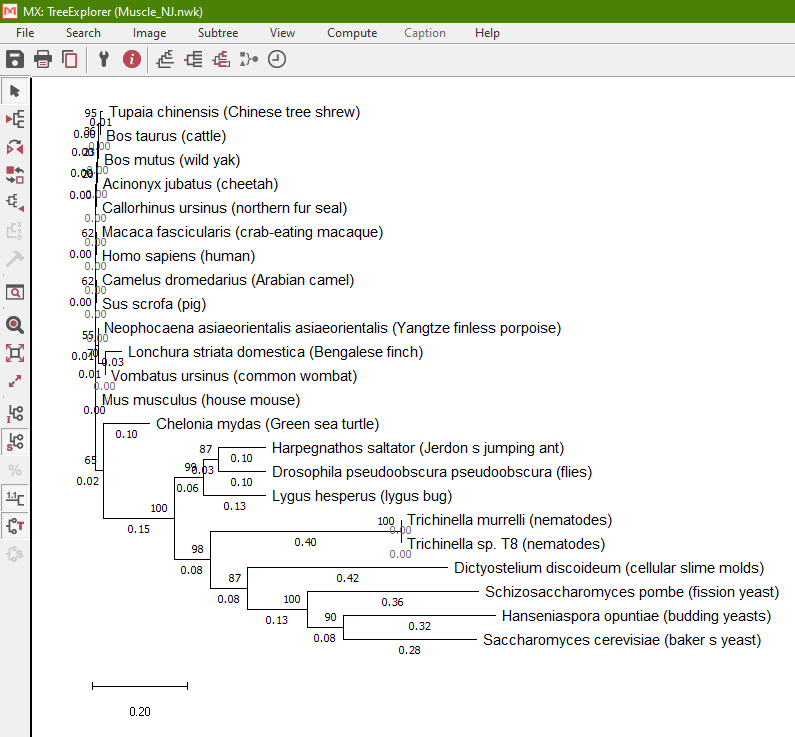
\includegraphics[width=.3\textwidth]{Muscle_NJ.png} &
      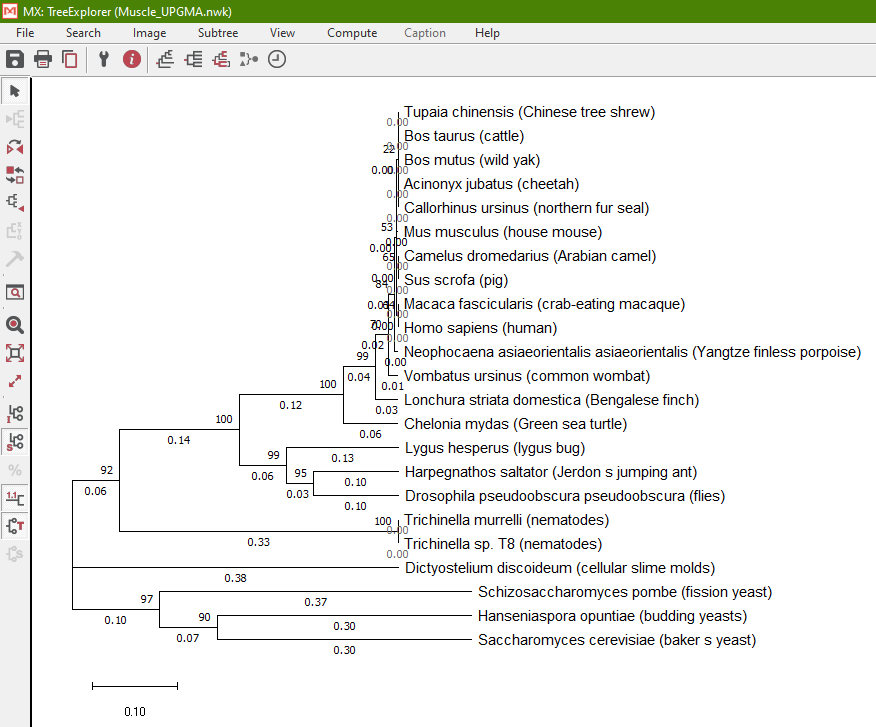
\includegraphics[width=.3\textwidth]{Muscle_UPGMA.png} \\\hline
      Метод Muscle и ML &
      Метод Muscle и NJ &
      Метод Muscle и UPGMA \\\hline
    \end{tabular}
  \end{center}

  \section{Выводы}
  Почему-то все деревья, построенные методами NJ (метод расстояний) и ML (метод максимального правдоподобия),
  получились совершенно неадекватными.
  Алгоритм, который работал 2 часа, в полной серьёзности утверждает что нематоды и дрожжи произошли от млекопитающих.
  Нормальными получились только деревья постойные методом UPGMA.

  \subsection{Одинаковая ли получилась топология деревьев при построении разными методами?}
  Все 3 метода построения деревьев дали совершенно разный результат, но только UPGMA получается хоть немного похож на правду.

  \subsection{Какой алгоритм выравнивания лучше сработал -- ClustalW или Muscle?}
  Вроде примерно одинаково (алгоритмы построения дерева влияют больше),
  но Muscle немного лучше, потому что сгруппировал дрожжи отдельно от животных.

  \subsection{Совпадают ли деревья, построенные по одному гену с принятыми деревьями видов?}
  Даже в самом правильном дереве нормально сгруппировать млекопитающих,
  потому что у них этот ген отличается очень мало, а у некоторых вообще совпадает.

  \subsection{Одинаковые ли получились бутстрэп-значения?}
  Бутстрэп-значения вообще везде получились разными.

  \section{Самое правильное дерево (бонус)}
  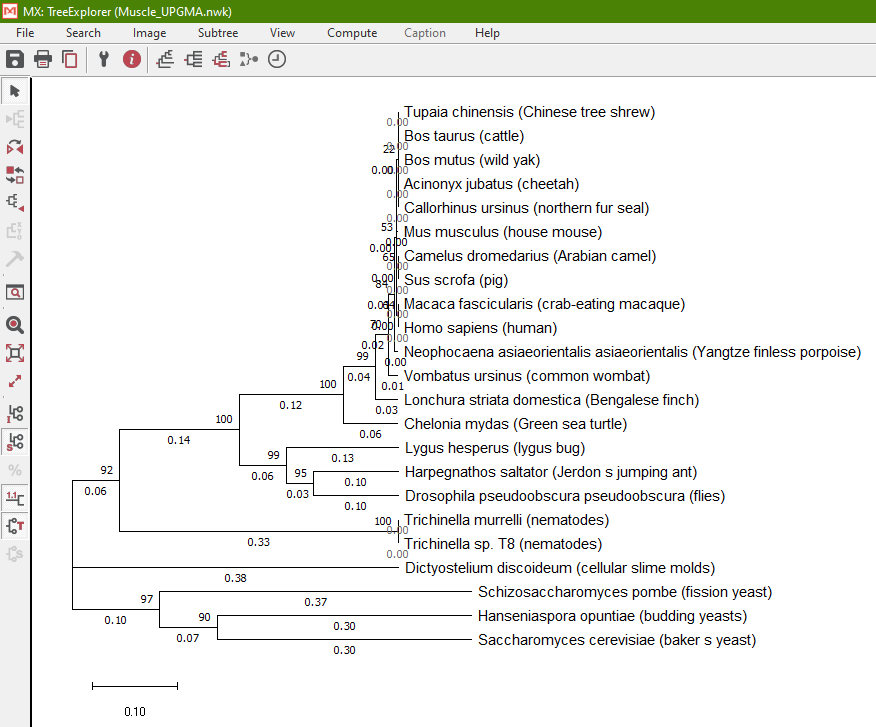
\includegraphics[width=\textwidth]{Muscle_UPGMA.png}


\end{document}
